\begin{minipage}{0.75\linewidth}
\begin{figure}[h]
    \centering
    \begin{adjustbox}{max width=1.0\linewidth, keepaspectratio}
        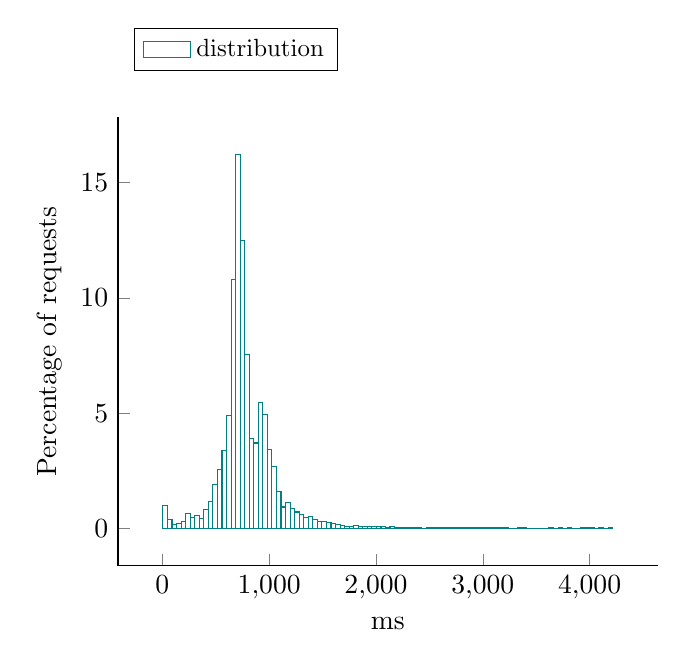
\begin{tikzpicture}
            \begin{axis}[ylabel = Percentage of requests, 
xlabel = ms, 
legend style = {nodes={scale=0.9, transform shape}, at={(0.03,1.2)}, anchor=north west, draw=black, fill=white, align=left, legend columns=3},
area style, mark size = 0pt,
 cycle list name = exotic,
  axis lines* = left]
		\addplot +[ybar interval] coordinates {
			 (5, 0.987629)
			 (47.53, 0.374259)
			 (90.06, 0.176734)
			 (132.59, 0.197526)
			 (175.12, 0.291091)
			 (217.65, 0.623765)
			 (260.18, 0.457428)
			 (302.71, 0.561389)
			 (345.24, 0.42624)
			 (387.77, 0.831687)
			 (430.3, 1.14357)
			 (472.83, 1.89209)
			 (515.36, 2.56783)
			 (557.89, 3.36833)
			 (600.42, 4.88616)
			 (642.95, 10.8119)
			 (685.48, 16.2179)
			 (728.01, 12.4753)
			 (770.54, 7.52677)
			 (813.07, 3.90893)
			 (855.6, 3.70101)
			 (898.13, 5.44755)
			 (940.66, 4.92775)
			 (983.19, 3.40992)
			 (1025.72, 2.6718)
			 (1068.25, 1.5906)
			 (1110.78, 0.925252)
			 (1153.31, 1.12278)
			 (1195.84, 0.842083)
			 (1238.37, 0.706934)
			 (1280.9, 0.582181)
			 (1323.43, 0.47822)
			 (1365.96, 0.530201)
			 (1408.49, 0.384655)
			 (1451.02, 0.280694)
			 (1493.55, 0.280694)
			 (1536.08, 0.259902)
			 (1578.61, 0.207922)
			 (1621.14, 0.166337)
			 (1663.67, 0.124753)
			 (1706.2, 0.0623765)
			 (1748.73, 0.0831687)
			 (1791.26, 0.114357)
			 (1833.79, 0.0935648)
			 (1876.32, 0.0727726)
			 (1918.85, 0.0623765)
			 (1961.38, 0.0727726)
			 (2003.91, 0.0831687)
			 (2046.44, 0.0623765)
			 (2088.97, 0.0207922)
			 (2131.5, 0.0623765)
			 (2174.03, 0.0415844)
			 (2216.56, 0.0311883)
			 (2259.09, 0.0415844)
			 (2301.62, 0.0415844)
			 (2344.15, 0.0311883)
			 (2386.68, 0.0207922)
			 (2429.21, 0)
			 (2471.74, 0.0415844)
			 (2514.27, 0.0207922)
			 (2556.8, 0.0415844)
			 (2599.33, 0.0207922)
			 (2641.86, 0.0311883)
			 (2684.39, 0.0103961)
			 (2726.92, 0.0311883)
			 (2769.45, 0.0207922)
			 (2811.98, 0.0415844)
			 (2854.51, 0.0207922)
			 (2897.04, 0.0207922)
			 (2939.57, 0.0311883)
			 (2982.1, 0.0415844)
			 (3024.63, 0.0311883)
			 (3067.16, 0.0103961)
			 (3109.69, 0.0103961)
			 (3152.22, 0.0207922)
			 (3194.75, 0.0103961)
			 (3237.28, 0)
			 (3279.81, 0)
			 (3322.34, 0.0103961)
			 (3364.87, 0.0103961)
			 (3407.4, 0)
			 (3449.93, 0)
			 (3492.46, 0)
			 (3534.99, 0)
			 (3577.52, 0)
			 (3620.05, 0.0103961)
			 (3662.58, 0)
			 (3705.11, 0.0103961)
			 (3747.64, 0)
			 (3790.17, 0.0415844)
			 (3832.7, 0)
			 (3875.23, 0)
			 (3917.76, 0.0103961)
			 (3960.29, 0.0207922)
			 (4002.82, 0.0207922)
			 (4045.35, 0)
			 (4087.88, 0.0103961)
			 (4130.41, 0)
			 (4172.94, 0.0103961)
			 (4215.47, 0.0103961)
		};
\addlegendentry{distribution};
           \end{axis}
      \end{tikzpicture}
  \end{adjustbox}
  \caption{Response time distribution - req = ReadUser-2}
\end{figure}
\end{minipage}\hfill\begin{minipage}{0.18\linewidth}
\begin{table}[h]
\begin{tabular}{|cc|}
\hline
\textbf{} & \textbf{ms}\\ \hline
 \Xhline{0.005\arrayrulewidth}
min & 5\\
 \Xhline{0.005\arrayrulewidth}
max & 4258\\
 \Xhline{0.005\arrayrulewidth}
mean & 800\\
 \Xhline{0.005\arrayrulewidth}
std & 324\\
\hline
\hline
 \Xhline{0.005\arrayrulewidth}
25th & 668\\
 \Xhline{0.005\arrayrulewidth}
50th & 741\\
 \Xhline{0.005\arrayrulewidth}
75th & 912\\
 \Xhline{0.005\arrayrulewidth}
80th & 948\\
 \Xhline{0.005\arrayrulewidth}
85th & 996\\
 \Xhline{0.005\arrayrulewidth}
90th & 1071\\
 \Xhline{0.005\arrayrulewidth}
95th & 1279\\
 \Xhline{0.005\arrayrulewidth}
99th & 2037\\
\hline
\end{tabular}
\caption{Response time}
\end{table}
\end{minipage}\hfill